\documentclass[aspectratio=169]{beamer}              % only frames

% for themes, etc.
\mode<presentation>
\usetheme{Madrid} 
\usecolortheme{crane}

%\usepackage{times}  % fonts are up to you
% The usual suspects
\usepackage{multirow, booktabs, dcolumn, color, graphicx} % Tables\usepackage{graphicx}
\usepackage{amsmath,amssymb,amsthm}
% Strikethrough text
\usepackage{soul}
% Adjust box to fit tabulars
\usepackage{adjustbox}
% Embed video
\usepackage{media9}
% For notes
\usepackage{pgfpages}
\setbeameroption{hide notes} % Only slides
%\setbeameroption{show only notes} % Only notes
%\setbeameroption{show notes on second screen=right} % Both
% Give a slight yellow tint to the notes page
%\setbeamertemplate{note page}{\pagecolor{yellow!5}\insertnote}\usepackage{palatino}
% Use colors by name
\usepackage{xcolor}
% EMBEDDING VIDEO IS POSSIBLE WITH PDFPC USE PDF PC to present
\usepackage{multimedia}



% The table highlighting for hypothesis discussion.
\usepackage[beamer,customcolors]{hf-tikz}
\usetikzlibrary{calc}

% To use background images
\newenvironment{colorframe}[2][]{%
\setbeamercolor{background canvas}{bg=#1}
\begin{frame}\color{white}}
{\end{frame}}


% To set the hypothesis highlighting boxes red.
\tikzset{hl/.style={
    set fill color=red!80!black!40,
    set border color=red!80!black,
  },
}

% Set Graphics folder
\graphicspath{{./figures/}}


% these will be used later in the title page
\title{Common Threats and Solutions}
\subtitle{Multifactor Authentication}
\author{Irfan Kanat}
\institute[CBS]{{Department of Digitization}\\ Copenhagen Business School}
\date{\today}



\begin{document}

% this prints title, author etc. info from above
\begin{frame}

	\titlepage

	\vfill
	{\tiny \centering This work is licensed under a \href{http://creativecommons.org/licenses/by/4.0/}{Creative Commons Attribution 4.0 International License}.}

\end{frame}

\note{In this video we will learn about multi factor authentication.}

\begin{frame}
	\frametitle{Authentication}
    
	Something you know \vspace{1em}

	Something you are \vspace{1em}

	Something you have

\end{frame}

\note{
	Three methods we use for authentication today are listed on this slide.

	For crucial accounts where security is important (official accounts, financial accounts, e-mails) it is a good idea to use more than one authentication method.

	So that if adversary circumvents one method, there is another that keeps us safe.
}


\begin{frame}
	\frametitle{Nem-ID}
    
	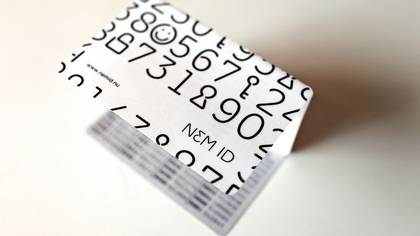
\includegraphics[width = \textwidth, height = .85\textheight, keepaspectratio]{figures/authenticator.jpeg}

\end{frame}

\begin{frame}
	\frametitle{Apps}
    
    \centering
    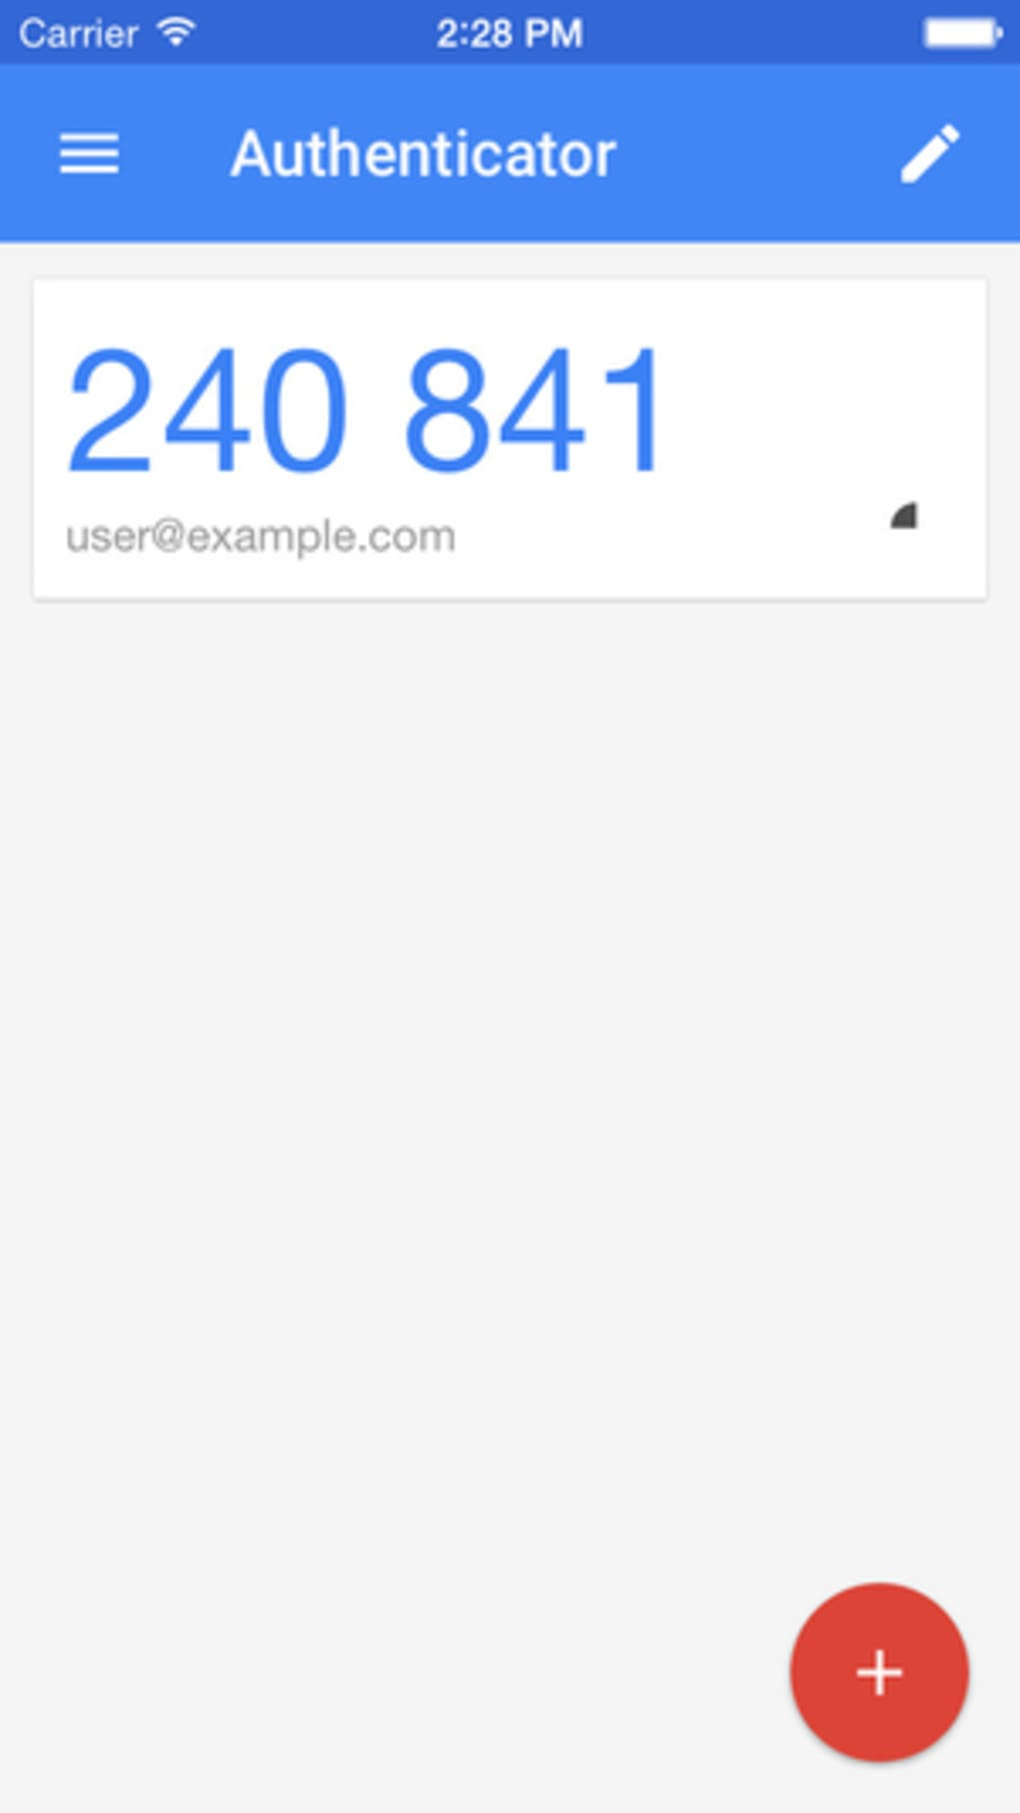
\includegraphics[width = \textwidth, height = .85\textheight, keepaspectratio]{figures/app.jpeg}

\end{frame}

\begin{frame}
	\frametitle{Hardware Keys}
    
    \centering	

    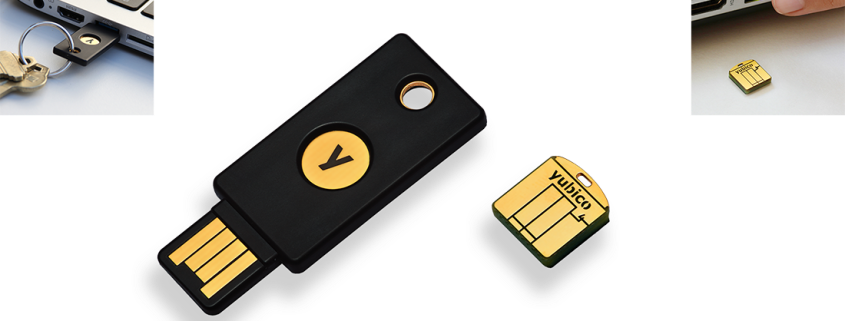
\includegraphics[width = \textwidth, height = .85\textheight, keepaspectratio]{figures/hardware.png}

\end{frame}

\begin{frame}
	\frametitle{2FA - MFA}
    
    Combining different methods increases security.

\end{frame}

\end{document}
